\documentclass[1p]{elsarticle_modified}
%\bibliographystyle{elsarticle-num}

%\usepackage[colorlinks]{hyperref}
%\usepackage{abbrmath_seonhwa} %\Abb, \Ascr, \Acal ,\Abf, \Afrak
\usepackage{amsfonts}
\usepackage{amssymb}
\usepackage{amsmath}
\usepackage{amsthm}
\usepackage{scalefnt}
\usepackage{amsbsy}
\usepackage{kotex}
\usepackage{caption}
\usepackage{subfig}
\usepackage{color}
\usepackage{graphicx}
\usepackage{xcolor} %% white, black, red, green, blue, cyan, magenta, yellow
\usepackage{float}
\usepackage{setspace}
\usepackage{hyperref}

\usepackage{tikz}
\usetikzlibrary{arrows}

\usepackage{multirow}
\usepackage{array} % fixed length table
\usepackage{hhline}

%%%%%%%%%%%%%%%%%%%%%
\makeatletter
\renewcommand*\env@matrix[1][\arraystretch]{%
	\edef\arraystretch{#1}%
	\hskip -\arraycolsep
	\let\@ifnextchar\new@ifnextchar
	\array{*\c@MaxMatrixCols c}}
\makeatother %https://tex.stackexchange.com/questions/14071/how-can-i-increase-the-line-spacing-in-a-matrix
%%%%%%%%%%%%%%%

\usepackage[normalem]{ulem}

\newcommand{\msout}[1]{\ifmmode\text{\sout{\ensuremath{#1}}}\else\sout{#1}\fi}
%SOURCE: \msout is \stkout macro in https://tex.stackexchange.com/questions/20609/strikeout-in-math-mode

\newcommand{\cancel}[1]{
	\ifmmode
	{\color{red}\msout{#1}}
	\else
	{\color{red}\sout{#1}}
	\fi
}

\newcommand{\add}[1]{
	{\color{blue}\uwave{#1}}
}

\newcommand{\replace}[2]{
	\ifmmode
	{\color{red}\msout{#1}}{\color{blue}\uwave{#2}}
	\else
	{\color{red}\sout{#1}}{\color{blue}\uwave{#2}}
	\fi
}

\newcommand{\Sol}{\mathcal{S}} %segment
\newcommand{\D}{D} %diagram
\newcommand{\A}{\mathcal{A}} %arc


%%%%%%%%%%%%%%%%%%%%%%%%%%%%%5 test

\def\sl{\operatorname{\textup{SL}}(2,\Cbb)}
\def\psl{\operatorname{\textup{PSL}}(2,\Cbb)}
\def\quan{\mkern 1mu \triangleright \mkern 1mu}

\theoremstyle{definition}
\newtheorem{thm}{Theorem}[section]
\newtheorem{prop}[thm]{Proposition}
\newtheorem{lem}[thm]{Lemma}
\newtheorem{ques}[thm]{Question}
\newtheorem{cor}[thm]{Corollary}
\newtheorem{defn}[thm]{Definition}
\newtheorem{exam}[thm]{Example}
\newtheorem{rmk}[thm]{Remark}
\newtheorem{alg}[thm]{Algorithm}

\newcommand{\I}{\sqrt{-1}}
\begin{document}

%\begin{frontmatter}
%
%\title{Boundary parabolic representations of knots up to 8 crossings}
%
%%% Group authors per affiliation:
%\author{Yunhi Cho} 
%\address{Department of Mathematics, University of Seoul, Seoul, Korea}
%\ead{yhcho@uos.ac.kr}
%
%
%\author{Seonhwa Kim} %\fnref{s_kim}}
%\address{Center for Geometry and Physics, Institute for Basic Science, Pohang, 37673, Korea}
%\ead{ryeona17@ibs.re.kr}
%
%\author{Hyuk Kim}
%\address{Department of Mathematical Sciences, Seoul National University, Seoul 08826, Korea}
%\ead{hyukkim@snu.ac.kr}
%
%\author{Seokbeom Yoon}
%\address{Department of Mathematical Sciences, Seoul National University, Seoul, 08826,  Korea}
%\ead{sbyoon15@snu.ac.kr}
%
%\begin{abstract}
%We find all boundary parabolic representation of knots up to 8 crossings.
%
%\end{abstract}
%\begin{keyword}
%    \MSC[2010] 57M25 
%\end{keyword}
%
%\end{frontmatter}

%\linenumbers
%\tableofcontents
%
\newcommand\colored[1]{\textcolor{white}{\rule[-0.35ex]{0.8em}{1.4ex}}\kern-0.8em\color{red} #1}%
%\newcommand\colored[1]{\textcolor{white}{ #1}\kern-2.17ex	\textcolor{white}{ #1}\kern-1.81ex	\textcolor{white}{ #1}\kern-2.15ex\color{red}#1	}

{\Large $\underline{11a_{42}~(K11a_{42})}$}

\setlength{\tabcolsep}{10pt}
\renewcommand{\arraystretch}{1.6}
\vspace{1cm}\begin{tabular}{m{100pt}>{\centering\arraybackslash}m{274pt}}
\multirow{5}{120pt}{
	\centering
	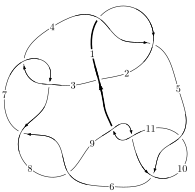
\includegraphics[width=112pt]{../../../GIT/diagram.site/Diagrams/png/291_11a_42.png}\\
\ \ \ A knot diagram\footnotemark}&
\allowdisplaybreaks
\textbf{Linearized knot diagam} \\
\cline{2-2}
 &
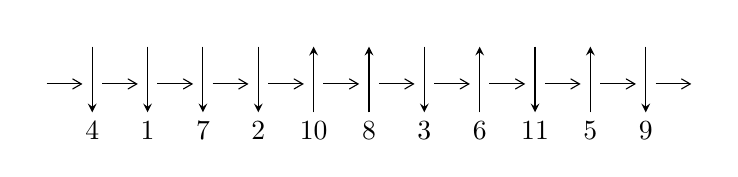
\begin{tikzpicture}[x=20pt, y=17pt]
	% nodes
	\node (C0) at (0, 0) {};
	\node (C1) at (1, 0) {};
	\node (C1U) at (1, +1) {};
	\node (C1D) at (1, -1) {4};

	\node (C2) at (2, 0) {};
	\node (C2U) at (2, +1) {};
	\node (C2D) at (2, -1) {1};

	\node (C3) at (3, 0) {};
	\node (C3U) at (3, +1) {};
	\node (C3D) at (3, -1) {7};

	\node (C4) at (4, 0) {};
	\node (C4U) at (4, +1) {};
	\node (C4D) at (4, -1) {2};

	\node (C5) at (5, 0) {};
	\node (C5U) at (5, +1) {};
	\node (C5D) at (5, -1) {10};

	\node (C6) at (6, 0) {};
	\node (C6U) at (6, +1) {};
	\node (C6D) at (6, -1) {8};

	\node (C7) at (7, 0) {};
	\node (C7U) at (7, +1) {};
	\node (C7D) at (7, -1) {3};

	\node (C8) at (8, 0) {};
	\node (C8U) at (8, +1) {};
	\node (C8D) at (8, -1) {6};

	\node (C9) at (9, 0) {};
	\node (C9U) at (9, +1) {};
	\node (C9D) at (9, -1) {11};

	\node (C10) at (10, 0) {};
	\node (C10U) at (10, +1) {};
	\node (C10D) at (10, -1) {5};

	\node (C11) at (11, 0) {};
	\node (C11U) at (11, +1) {};
	\node (C11D) at (11, -1) {9};
	\node (C12) at (12, 0) {};

	% arrows
	\draw[->,>={angle 60}]
	(C0) edge (C1) (C1) edge (C2) (C2) edge (C3) (C3) edge (C4) (C4) edge (C5) (C5) edge (C6) (C6) edge (C7) (C7) edge (C8) (C8) edge (C9) (C9) edge (C10) (C10) edge (C11) (C11) edge (C12) ;	\draw[->,>=stealth]
	(C1U) edge (C1D) (C2U) edge (C2D) (C3U) edge (C3D) (C4U) edge (C4D) (C5D) edge (C5U) (C6D) edge (C6U) (C7U) edge (C7D) (C8D) edge (C8U) (C9U) edge (C9D) (C10D) edge (C10U) (C11U) edge (C11D) ;
	\end{tikzpicture} \\
\hhline{~~} \\& 
\textbf{Solving Sequence} \\ \cline{2-2} 
 &
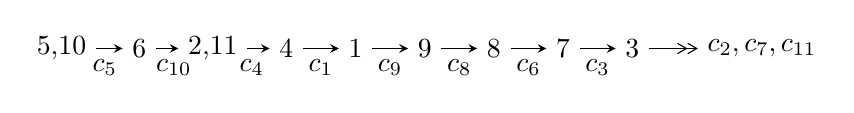
\begin{tikzpicture}[x=25pt, y=7pt]
	% node
	\node (A0) at (-1/8, 0) {5,10};
	\node (A1) at (1, 0) {6};
	\node (A2) at (33/16, 0) {2,11};
	\node (A3) at (25/8, 0) {4};
	\node (A4) at (33/8, 0) {1};
	\node (A5) at (41/8, 0) {9};
	\node (A6) at (49/8, 0) {8};
	\node (A7) at (57/8, 0) {7};
	\node (A8) at (65/8, 0) {3};
	\node (C1) at (1/2, -1) {$c_{5}$};
	\node (C2) at (3/2, -1) {$c_{10}$};
	\node (C3) at (21/8, -1) {$c_{4}$};
	\node (C4) at (29/8, -1) {$c_{1}$};
	\node (C5) at (37/8, -1) {$c_{9}$};
	\node (C6) at (45/8, -1) {$c_{8}$};
	\node (C7) at (53/8, -1) {$c_{6}$};
	\node (C8) at (61/8, -1) {$c_{3}$};
	\node (A9) at (10, 0) {$c_{2},c_{7},c_{11}$};

	% edge
	\draw[->,>=stealth]	
	(A0) edge (A1) (A1) edge (A2) (A2) edge (A3) (A3) edge (A4) (A4) edge (A5) (A5) edge (A6) (A6) edge (A7) (A7) edge (A8) ;
	\draw[->>,>={angle 60}]	
	(A8) edge (A9);
\end{tikzpicture} \\ 

\end{tabular} \\

\footnotetext{
The image of knot diagram is generated by the software ``\textbf{Draw programme}" developed by Andrew Bartholomew(\url{http://www.layer8.co.uk/maths/draw/index.htm\#Running-draw}), where we modified some parts for our purpose(\url{https://github.com/CATsTAILs/LinksPainter}).
}\phantom \\ \newline 
\centering \textbf{Ideals for irreducible components\footnotemark of $X_{\text{par}}$} 
 
\begin{align*}
I^u_{1}&=\langle 
u^{53}+u^{52}+\cdots+b+1,\;- u^{54}- u^{53}+\cdots+a-1,\;u^{55}+2 u^{54}+\cdots+2 u+1\rangle \\
I^u_{2}&=\langle 
b+1,\;a- u+1,\;u^2+u+1\rangle \\
\\
\end{align*}
\raggedright * 2 irreducible components of $\dim_{\mathbb{C}}=0$, with total 57 representations.\\
\footnotetext{All coefficients of polynomials are rational numbers. But the coefficients are sometimes approximated in decimal forms when there is not enough margin.}
\newpage
\renewcommand{\arraystretch}{1}
\centering \section*{I. $I^u_{1}= \langle u^{53}+u^{52}+\cdots+b+1,\;- u^{54}- u^{53}+\cdots+a-1,\;u^{55}+2 u^{54}+\cdots+2 u+1 \rangle$}
\flushleft \textbf{(i) Arc colorings}\\
\begin{tabular}{m{7pt} m{180pt} m{7pt} m{180pt} }
\flushright $a_{5}=$&$\begin{pmatrix}1\\0\end{pmatrix}$ \\
\flushright $a_{10}=$&$\begin{pmatrix}0\\u\end{pmatrix}$ \\
\flushright $a_{6}=$&$\begin{pmatrix}1\\- u^2\end{pmatrix}$ \\
\flushright $a_{2}=$&$\begin{pmatrix}u^{54}+u^{53}+\cdots-3 u+1\\- u^{53}- u^{52}+\cdots+u-1\end{pmatrix}$ \\
\flushright $a_{11}=$&$\begin{pmatrix}u\\u\end{pmatrix}$ \\
\flushright $a_{4}=$&$\begin{pmatrix}u^{54}+9 u^{52}+\cdots-4 u+1\\- u^{53}- u^{52}+\cdots+u^2-1\end{pmatrix}$ \\
\flushright $a_{1}=$&$\begin{pmatrix}u^5+u\\u^5+u^3+u\end{pmatrix}$ \\
\flushright $a_{9}=$&$\begin{pmatrix}u^3\\u^3+u\end{pmatrix}$ \\
\flushright $a_{8}=$&$\begin{pmatrix}- u^5- u\\u^7+u^5+2 u^3+u\end{pmatrix}$ \\
\flushright $a_{7}=$&$\begin{pmatrix}u^{10}+u^8+2 u^6+u^4+u^2+1\\- u^{12}-2 u^{10}-4 u^8-4 u^6-3 u^4-2 u^2\end{pmatrix}$ \\
\flushright $a_{3}=$&$\begin{pmatrix}u^{54}+2 u^{53}+\cdots-2 u+2\\- u^{53}- u^{52}+\cdots+u-1\end{pmatrix}$\\ \flushright $a_{3}=$&$\begin{pmatrix}u^{54}+2 u^{53}+\cdots-2 u+2\\- u^{53}- u^{52}+\cdots+u-1\end{pmatrix}$\\&\end{tabular}
\flushleft \textbf{(ii) Obstruction class $= -1$}\\~\\
\flushleft \textbf{(iii) Cusp Shapes $= u^{54}-7 u^{53}+\cdots- u-10$}\\~\\
\newpage\renewcommand{\arraystretch}{1}
\flushleft \textbf{(iv) u-Polynomials at the component}\newline \\
\begin{tabular}{m{50pt}|m{274pt}}
Crossings & \hspace{64pt}u-Polynomials at each crossing \\
\hline $$\begin{aligned}c_{1},c_{4}\end{aligned}$$&$\begin{aligned}
&u^{55}-3 u^{54}+\cdots-5 u+1
\end{aligned}$\\
\hline $$\begin{aligned}c_{2}\end{aligned}$$&$\begin{aligned}
&u^{55}+31 u^{54}+\cdots-7 u+1
\end{aligned}$\\
\hline $$\begin{aligned}c_{3},c_{7}\end{aligned}$$&$\begin{aligned}
&u^{55}+u^{54}+\cdots+8 u+4
\end{aligned}$\\
\hline $$\begin{aligned}c_{5},c_{10}\end{aligned}$$&$\begin{aligned}
&u^{55}+2 u^{54}+\cdots+2 u+1
\end{aligned}$\\
\hline $$\begin{aligned}c_{6},c_{8}\end{aligned}$$&$\begin{aligned}
&u^{55}-15 u^{54}+\cdots-168 u+16
\end{aligned}$\\
\hline $$\begin{aligned}c_{9},c_{11}\end{aligned}$$&$\begin{aligned}
&u^{55}+20 u^{54}+\cdots+14 u-1
\end{aligned}$\\
\hline
\end{tabular}\\~\\
\newpage\renewcommand{\arraystretch}{1}
\flushleft \textbf{(v) Riley Polynomials at the component}\newline \\
\begin{tabular}{m{50pt}|m{274pt}}
Crossings & \hspace{64pt}Riley Polynomials at each crossing \\
\hline $$\begin{aligned}c_{1},c_{4}\end{aligned}$$&$\begin{aligned}
&y^{55}-31 y^{54}+\cdots-7 y-1
\end{aligned}$\\
\hline $$\begin{aligned}c_{2}\end{aligned}$$&$\begin{aligned}
&y^{55}-11 y^{54}+\cdots+101 y-1
\end{aligned}$\\
\hline $$\begin{aligned}c_{3},c_{7}\end{aligned}$$&$\begin{aligned}
&y^{55}+15 y^{54}+\cdots-168 y-16
\end{aligned}$\\
\hline $$\begin{aligned}c_{5},c_{10}\end{aligned}$$&$\begin{aligned}
&y^{55}+20 y^{54}+\cdots+14 y-1
\end{aligned}$\\
\hline $$\begin{aligned}c_{6},c_{8}\end{aligned}$$&$\begin{aligned}
&y^{55}+47 y^{54}+\cdots+3616 y-256
\end{aligned}$\\
\hline $$\begin{aligned}c_{9},c_{11}\end{aligned}$$&$\begin{aligned}
&y^{55}+32 y^{54}+\cdots+490 y-1
\end{aligned}$\\
\hline
\end{tabular}\\~\\
\newpage\flushleft \textbf{(vi) Complex Volumes and Cusp Shapes}
$$\begin{array}{c|c|c}  
\text{Solutions to }I^u_{1}& \I (\text{vol} + \sqrt{-1}CS) & \text{Cusp shape}\\
 \hline 
\begin{aligned}
u &= -0.816179 + 0.574717 I \\
a &= \phantom{-}1.027890 + 0.674902 I \\
b &= \phantom{-}1.204850 - 0.521092 I\end{aligned}
 & -2.90431 + 8.91686 I & -3.42760 - 5.44869 I \\ \hline\begin{aligned}
u &= -0.816179 - 0.574717 I \\
a &= \phantom{-}1.027890 - 0.674902 I \\
b &= \phantom{-}1.204850 + 0.521092 I\end{aligned}
 & -2.90431 - 8.91686 I & -3.42760 + 5.44869 I \\ \hline\begin{aligned}
u &= \phantom{-}0.239129 + 0.986379 I \\
a &= \phantom{-}2.23250 + 0.41423 I \\
b &= \phantom{-}0.941364 - 0.397946 I\end{aligned}
 & -1.92448 + 4.39584 I & -6.07569 - 8.49319 I \\ \hline\begin{aligned}
u &= \phantom{-}0.239129 - 0.986379 I \\
a &= \phantom{-}2.23250 - 0.41423 I \\
b &= \phantom{-}0.941364 + 0.397946 I\end{aligned}
 & -1.92448 - 4.39584 I & -6.07569 + 8.49319 I \\ \hline\begin{aligned}
u &= -0.779335 + 0.590843 I \\
a &= \phantom{-}0.007618 - 0.199836 I \\
b &= \phantom{-}0.147161 + 0.837390 I\end{aligned}
 & \phantom{-}0.24633 + 3.95028 I & -0.20932 - 2.43300 I \\ \hline\begin{aligned}
u &= -0.779335 - 0.590843 I \\
a &= \phantom{-}0.007618 + 0.199836 I \\
b &= \phantom{-}0.147161 - 0.837390 I\end{aligned}
 & \phantom{-}0.24633 - 3.95028 I & -0.20932 + 2.43300 I \\ \hline\begin{aligned}
u &= \phantom{-}0.658398 + 0.801536 I \\
a &= \phantom{-}0.867357 + 0.882946 I \\
b &= -0.733611 - 0.391605 I\end{aligned}
 & \phantom{-}0.872499 + 0.772147 I & -1.84032 + 0.30762 I \\ \hline\begin{aligned}
u &= \phantom{-}0.658398 - 0.801536 I \\
a &= \phantom{-}0.867357 - 0.882946 I \\
b &= -0.733611 + 0.391605 I\end{aligned}
 & \phantom{-}0.872499 - 0.772147 I & -1.84032 - 0.30762 I \\ \hline\begin{aligned}
u &= \phantom{-}0.759593 + 0.559351 I \\
a &= -1.09162 + 0.93530 I \\
b &= -1.176880 - 0.449966 I\end{aligned}
 & -3.79702 - 2.69601 I & -4.74745 + 1.11286 I \\ \hline\begin{aligned}
u &= \phantom{-}0.759593 - 0.559351 I \\
a &= -1.09162 - 0.93530 I \\
b &= -1.176880 + 0.449966 I\end{aligned}
 & -3.79702 + 2.69601 I & -4.74745 - 1.11286 I\\
 \hline 
 \end{array}$$\newpage$$\begin{array}{c|c|c}  
\text{Solutions to }I^u_{1}& \I (\text{vol} + \sqrt{-1}CS) & \text{Cusp shape}\\
 \hline 
\begin{aligned}
u &= -0.628216 + 0.858582 I \\
a &= -1.51296 + 0.91306 I \\
b &= -1.203820 + 0.035992 I\end{aligned}
 & -0.64263 - 2.45826 I & \phantom{-0.000000 -}0. + 4.47694 I \\ \hline\begin{aligned}
u &= -0.628216 - 0.858582 I \\
a &= -1.51296 - 0.91306 I \\
b &= -1.203820 - 0.035992 I\end{aligned}
 & -0.64263 + 2.45826 I & \phantom{-0.000000 } 0. - 4.47694 I \\ \hline\begin{aligned}
u &= \phantom{-}0.451120 + 0.966547 I \\
a &= \phantom{-}1.27088 + 0.78560 I \\
b &= \phantom{-}0.763301 + 0.197825 I\end{aligned}
 & -0.85220 + 1.53742 I & -0.475415 + 0.770388 I \\ \hline\begin{aligned}
u &= \phantom{-}0.451120 - 0.966547 I \\
a &= \phantom{-}1.27088 - 0.78560 I \\
b &= \phantom{-}0.763301 - 0.197825 I\end{aligned}
 & -0.85220 - 1.53742 I & -0.475415 - 0.770388 I \\ \hline\begin{aligned}
u &= -0.761308 + 0.748686 I \\
a &= \phantom{-}0.068239 + 0.640254 I \\
b &= \phantom{-}0.916664 - 0.588628 I\end{aligned}
 & \phantom{-}4.30983 + 3.18273 I & \phantom{-}1.66711 - 3.75336 I \\ \hline\begin{aligned}
u &= -0.761308 - 0.748686 I \\
a &= \phantom{-}0.068239 - 0.640254 I \\
b &= \phantom{-}0.916664 + 0.588628 I\end{aligned}
 & \phantom{-}4.30983 - 3.18273 I & \phantom{-}1.66711 + 3.75336 I \\ \hline\begin{aligned}
u &= -0.735974 + 0.536493 I \\
a &= -1.28675 + 0.70502 I \\
b &= -1.228780 - 0.367943 I\end{aligned}
 & -3.97885 - 0.10775 I & -4.88979 + 0.08750 I \\ \hline\begin{aligned}
u &= -0.735974 - 0.536493 I \\
a &= -1.28675 - 0.70502 I \\
b &= -1.228780 + 0.367943 I\end{aligned}
 & -3.97885 + 0.10775 I & -4.88979 - 0.08750 I \\ \hline\begin{aligned}
u &= -0.740147 + 0.806502 I \\
a &= \phantom{-}0.213975 - 0.919578 I \\
b &= \phantom{-}0.579824 + 0.662419 I\end{aligned}
 & \phantom{-}5.27340 - 1.63575 I & \phantom{-}3.78529 + 2.66903 I \\ \hline\begin{aligned}
u &= -0.740147 - 0.806502 I \\
a &= \phantom{-}0.213975 + 0.919578 I \\
b &= \phantom{-}0.579824 - 0.662419 I\end{aligned}
 & \phantom{-}5.27340 + 1.63575 I & \phantom{-}3.78529 - 2.66903 I\\
 \hline 
 \end{array}$$\newpage$$\begin{array}{c|c|c}  
\text{Solutions to }I^u_{1}& \I (\text{vol} + \sqrt{-1}CS) & \text{Cusp shape}\\
 \hline 
\begin{aligned}
u &= \phantom{-}0.034329 + 1.104990 I \\
a &= \phantom{-}0.080168 + 1.136900 I \\
b &= \phantom{-}0.053635 + 0.828871 I\end{aligned}
 & -5.60698 + 2.95534 I & -7.15421 - 2.80412 I \\ \hline\begin{aligned}
u &= \phantom{-}0.034329 - 1.104990 I \\
a &= \phantom{-}0.080168 - 1.136900 I \\
b &= \phantom{-}0.053635 - 0.828871 I\end{aligned}
 & -5.60698 - 2.95534 I & -7.15421 + 2.80412 I \\ \hline\begin{aligned}
u &= -0.009089 + 1.113840 I \\
a &= -3.11350 + 0.11167 I \\
b &= -1.231540 - 0.429492 I\end{aligned}
 & -9.45702 - 1.46557 I & -10.98966 + 0. I\phantom{ +0.000000I} \\ \hline\begin{aligned}
u &= -0.009089 - 1.113840 I \\
a &= -3.11350 - 0.11167 I \\
b &= -1.231540 + 0.429492 I\end{aligned}
 & -9.45702 + 1.46557 I & -10.98966 + 0. I\phantom{ +0.000000I} \\ \hline\begin{aligned}
u &= \phantom{-}0.660868 + 0.897456 I \\
a &= -0.21776 - 2.20899 I \\
b &= -0.826919 + 0.421607 I\end{aligned}
 & \phantom{-}0.57728 + 4.35301 I & -2.97848 - 6.56505 I \\ \hline\begin{aligned}
u &= \phantom{-}0.660868 - 0.897456 I \\
a &= -0.21776 + 2.20899 I \\
b &= -0.826919 - 0.421607 I\end{aligned}
 & \phantom{-}0.57728 - 4.35301 I & -2.97848 + 6.56505 I \\ \hline\begin{aligned}
u &= \phantom{-}0.757497 + 0.440100 I \\
a &= \phantom{-}1.156460 + 0.615207 I \\
b &= \phantom{-}1.177720 - 0.463008 I\end{aligned}
 & -3.70073 + 5.77207 I & -4.07257 - 5.94241 I \\ \hline\begin{aligned}
u &= \phantom{-}0.757497 - 0.440100 I \\
a &= \phantom{-}1.156460 - 0.615207 I \\
b &= \phantom{-}1.177720 + 0.463008 I\end{aligned}
 & -3.70073 - 5.77207 I & -4.07257 + 5.94241 I \\ \hline\begin{aligned}
u &= \phantom{-}0.047537 + 1.140170 I \\
a &= \phantom{-}2.98663 + 0.01514 I \\
b &= \phantom{-}1.219040 - 0.483533 I\end{aligned}
 & -9.06604 + 7.69131 I & -10.03059 - 5.89654 I \\ \hline\begin{aligned}
u &= \phantom{-}0.047537 - 1.140170 I \\
a &= \phantom{-}2.98663 - 0.01514 I \\
b &= \phantom{-}1.219040 + 0.483533 I\end{aligned}
 & -9.06604 - 7.69131 I & -10.03059 + 5.89654 I\\
 \hline 
 \end{array}$$\newpage$$\begin{array}{c|c|c}  
\text{Solutions to }I^u_{1}& \I (\text{vol} + \sqrt{-1}CS) & \text{Cusp shape}\\
 \hline 
\begin{aligned}
u &= -0.718549 + 0.906381 I \\
a &= -0.652105 + 0.027561 I \\
b &= \phantom{-}0.517863 - 0.687312 I\end{aligned}
 & \phantom{-}4.96946 - 3.90710 I & \phantom{-0.000000 } 0 \\ \hline\begin{aligned}
u &= -0.718549 - 0.906381 I \\
a &= -0.652105 - 0.027561 I \\
b &= \phantom{-}0.517863 + 0.687312 I\end{aligned}
 & \phantom{-}4.96946 + 3.90710 I & \phantom{-0.000000 } 0 \\ \hline\begin{aligned}
u &= \phantom{-}0.669924 + 0.499239 I \\
a &= \phantom{-}0.164189 - 0.143161 I \\
b &= \phantom{-}0.025988 + 0.692151 I\end{aligned}
 & -0.47649 + 1.47491 I & -0.96799 - 2.91910 I \\ \hline\begin{aligned}
u &= \phantom{-}0.669924 - 0.499239 I \\
a &= \phantom{-}0.164189 + 0.143161 I \\
b &= \phantom{-}0.025988 - 0.692151 I\end{aligned}
 & -0.47649 - 1.47491 I & -0.96799 + 2.91910 I \\ \hline\begin{aligned}
u &= -0.717366 + 0.952779 I \\
a &= \phantom{-}1.15907 - 1.72863 I \\
b &= \phantom{-}0.963009 + 0.589107 I\end{aligned}
 & \phantom{-}3.69457 - 8.78385 I & \phantom{-0.000000 } 0 \\ \hline\begin{aligned}
u &= -0.717366 - 0.952779 I \\
a &= \phantom{-}1.15907 + 1.72863 I \\
b &= \phantom{-}0.963009 - 0.589107 I\end{aligned}
 & \phantom{-}3.69457 + 8.78385 I & \phantom{-0.000000 } 0 \\ \hline\begin{aligned}
u &= \phantom{-}0.629765 + 1.027960 I \\
a &= \phantom{-}1.069910 - 0.306602 I \\
b &= -0.051867 - 0.757851 I\end{aligned}
 & -1.91291 + 3.57990 I & \phantom{-0.000000 } 0 \\ \hline\begin{aligned}
u &= \phantom{-}0.629765 - 1.027960 I \\
a &= \phantom{-}1.069910 + 0.306602 I \\
b &= -0.051867 + 0.757851 I\end{aligned}
 & -1.91291 - 3.57990 I & \phantom{-0.000000 } 0 \\ \hline\begin{aligned}
u &= \phantom{-}0.362022 + 0.691095 I \\
a &= \phantom{-}0.432775 + 0.109549 I \\
b &= \phantom{-}0.059148 + 0.370271 I\end{aligned}
 & -0.194248 + 1.398020 I & -2.04153 - 4.84692 I \\ \hline\begin{aligned}
u &= \phantom{-}0.362022 - 0.691095 I \\
a &= \phantom{-}0.432775 - 0.109549 I \\
b &= \phantom{-}0.059148 - 0.370271 I\end{aligned}
 & -0.194248 - 1.398020 I & -2.04153 + 4.84692 I\\
 \hline 
 \end{array}$$\newpage$$\begin{array}{c|c|c}  
\text{Solutions to }I^u_{1}& \I (\text{vol} + \sqrt{-1}CS) & \text{Cusp shape}\\
 \hline 
\begin{aligned}
u &= -0.647113 + 1.040820 I \\
a &= -1.50753 + 1.09395 I \\
b &= -1.261440 + 0.376282 I\end{aligned}
 & -5.43130 - 5.17320 I & \phantom{-0.000000 } 0 \\ \hline\begin{aligned}
u &= -0.647113 - 1.040820 I \\
a &= -1.50753 - 1.09395 I \\
b &= -1.261440 - 0.376282 I\end{aligned}
 & -5.43130 + 5.17320 I & \phantom{-0.000000 } 0 \\ \hline\begin{aligned}
u &= \phantom{-}0.612711 + 1.063030 I \\
a &= \phantom{-}1.45098 + 1.12168 I \\
b &= \phantom{-}1.194960 + 0.434256 I\end{aligned}
 & -5.49641 - 0.62899 I & \phantom{-0.000000 } 0 \\ \hline\begin{aligned}
u &= \phantom{-}0.612711 - 1.063030 I \\
a &= \phantom{-}1.45098 - 1.12168 I \\
b &= \phantom{-}1.194960 - 0.434256 I\end{aligned}
 & -5.49641 + 0.62899 I & \phantom{-0.000000 } 0 \\ \hline\begin{aligned}
u &= \phantom{-}0.659279 + 1.042970 I \\
a &= -2.25573 - 2.04389 I \\
b &= -1.193240 + 0.473729 I\end{aligned}
 & -5.21292 + 8.08647 I & \phantom{-0.000000 } 0 \\ \hline\begin{aligned}
u &= \phantom{-}0.659279 - 1.042970 I \\
a &= -2.25573 + 2.04389 I \\
b &= -1.193240 - 0.473729 I\end{aligned}
 & -5.21292 - 8.08647 I & \phantom{-0.000000 } 0 \\ \hline\begin{aligned}
u &= -0.674581 + 1.040260 I \\
a &= -0.956881 - 0.394384 I \\
b &= \phantom{-}0.134773 - 0.873581 I\end{aligned}
 & -1.08802 - 9.45303 I & \phantom{-0.000000 } 0 \\ \hline\begin{aligned}
u &= -0.674581 - 1.040260 I \\
a &= -0.956881 + 0.394384 I \\
b &= \phantom{-}0.134773 + 0.873581 I\end{aligned}
 & -1.08802 + 9.45303 I & \phantom{-0.000000 } 0 \\ \hline\begin{aligned}
u &= -0.088965 + 0.747457 I \\
a &= -2.45827 + 1.39779 I \\
b &= -1.051280 - 0.242889 I\end{aligned}
 & -3.08639 - 0.93841 I & -10.69919 - 0.06174 I \\ \hline\begin{aligned}
u &= -0.088965 - 0.747457 I \\
a &= -2.45827 - 1.39779 I \\
b &= -1.051280 + 0.242889 I\end{aligned}
 & -3.08639 + 0.93841 I & -10.69919 + 0.06174 I\\
 \hline 
 \end{array}$$\newpage$$\begin{array}{c|c|c}  
\text{Solutions to }I^u_{1}& \I (\text{vol} + \sqrt{-1}CS) & \text{Cusp shape}\\
 \hline 
\begin{aligned}
u &= -0.681167 + 1.057900 I \\
a &= \phantom{-}2.24142 - 1.78647 I \\
b &= \phantom{-}1.221340 + 0.526305 I\end{aligned}
 & -4.3508 - 14.5336 I & \phantom{-0.000000 } 0 \\ \hline\begin{aligned}
u &= -0.681167 - 1.057900 I \\
a &= \phantom{-}2.24142 + 1.78647 I \\
b &= \phantom{-}1.221340 - 0.526305 I\end{aligned}
 & -4.3508 + 14.5336 I & \phantom{-0.000000 } 0 \\ \hline\begin{aligned}
u &= \phantom{-}0.561929 + 0.106681 I \\
a &= \phantom{-}0.365566 + 0.579622 I \\
b &= \phantom{-}0.769448 - 0.437822 I\end{aligned}
 & \phantom{-}1.33757 + 1.88655 I & \phantom{-}2.60483 - 4.69845 I \\ \hline\begin{aligned}
u &= \phantom{-}0.561929 - 0.106681 I \\
a &= \phantom{-}0.365566 - 0.579622 I \\
b &= \phantom{-}0.769448 + 0.437822 I\end{aligned}
 & \phantom{-}1.33757 - 1.88655 I & \phantom{-}2.60483 + 4.69845 I \\ \hline\begin{aligned}
u &= -0.212225\phantom{ +0.000000I} \\
a &= \phantom{-}2.51493\phantom{ +0.000000I} \\
b &= -0.861415\phantom{ +0.000000I}\end{aligned}
 & -1.25349\phantom{ +0.000000I} & -8.32260\phantom{ +0.000000I}\\
 \hline 
 \end{array}$$\newpage\newpage\renewcommand{\arraystretch}{1}
\centering \section*{II. $I^u_{2}= \langle b+1,\;a- u+1,\;u^2+u+1 \rangle$}
\flushleft \textbf{(i) Arc colorings}\\
\begin{tabular}{m{7pt} m{180pt} m{7pt} m{180pt} }
\flushright $a_{5}=$&$\begin{pmatrix}1\\0\end{pmatrix}$ \\
\flushright $a_{10}=$&$\begin{pmatrix}0\\u\end{pmatrix}$ \\
\flushright $a_{6}=$&$\begin{pmatrix}1\\u+1\end{pmatrix}$ \\
\flushright $a_{2}=$&$\begin{pmatrix}u-1\\-1\end{pmatrix}$ \\
\flushright $a_{11}=$&$\begin{pmatrix}u\\u\end{pmatrix}$ \\
\flushright $a_{4}=$&$\begin{pmatrix}u\\-1\end{pmatrix}$ \\
\flushright $a_{1}=$&$\begin{pmatrix}-1\\0\end{pmatrix}$ \\
\flushright $a_{9}=$&$\begin{pmatrix}1\\u+1\end{pmatrix}$ \\
\flushright $a_{8}=$&$\begin{pmatrix}1\\u+1\end{pmatrix}$ \\
\flushright $a_{7}=$&$\begin{pmatrix}1\\u+1\end{pmatrix}$ \\
\flushright $a_{3}=$&$\begin{pmatrix}u\\-1\end{pmatrix}$\\ \flushright $a_{3}=$&$\begin{pmatrix}u\\-1\end{pmatrix}$\\&\end{tabular}
\flushleft \textbf{(ii) Obstruction class $= 1$}\\~\\
\flushleft \textbf{(iii) Cusp Shapes $= 4 u-7$}\\~\\
\newpage\renewcommand{\arraystretch}{1}
\flushleft \textbf{(iv) u-Polynomials at the component}\newline \\
\begin{tabular}{m{50pt}|m{274pt}}
Crossings & \hspace{64pt}u-Polynomials at each crossing \\
\hline $$\begin{aligned}c_{1}\end{aligned}$$&$\begin{aligned}
&(u-1)^2
\end{aligned}$\\
\hline $$\begin{aligned}c_{2},c_{4}\end{aligned}$$&$\begin{aligned}
&(u+1)^2
\end{aligned}$\\
\hline $$\begin{aligned}c_{3},c_{6},c_{7}\\c_{8}\end{aligned}$$&$\begin{aligned}
&u^2
\end{aligned}$\\
\hline $$\begin{aligned}c_{5},c_{11}\end{aligned}$$&$\begin{aligned}
&u^2+u+1
\end{aligned}$\\
\hline $$\begin{aligned}c_{9},c_{10}\end{aligned}$$&$\begin{aligned}
&u^2- u+1
\end{aligned}$\\
\hline
\end{tabular}\\~\\
\newpage\renewcommand{\arraystretch}{1}
\flushleft \textbf{(v) Riley Polynomials at the component}\newline \\
\begin{tabular}{m{50pt}|m{274pt}}
Crossings & \hspace{64pt}Riley Polynomials at each crossing \\
\hline $$\begin{aligned}c_{1},c_{2},c_{4}\end{aligned}$$&$\begin{aligned}
&(y-1)^2
\end{aligned}$\\
\hline $$\begin{aligned}c_{3},c_{6},c_{7}\\c_{8}\end{aligned}$$&$\begin{aligned}
&y^2
\end{aligned}$\\
\hline $$\begin{aligned}c_{5},c_{9},c_{10}\\c_{11}\end{aligned}$$&$\begin{aligned}
&y^2+y+1
\end{aligned}$\\
\hline
\end{tabular}\\~\\
\newpage\flushleft \textbf{(vi) Complex Volumes and Cusp Shapes}
$$\begin{array}{c|c|c}  
\text{Solutions to }I^u_{2}& \I (\text{vol} + \sqrt{-1}CS) & \text{Cusp shape}\\
 \hline 
\begin{aligned}
u &= -0.500000 + 0.866025 I \\
a &= -1.50000 + 0.86603 I \\
b &= -1.00000\phantom{ +0.000000I}\end{aligned}
 & -1.64493 - 2.02988 I & -9.00000 + 3.46410 I \\ \hline\begin{aligned}
u &= -0.500000 - 0.866025 I \\
a &= -1.50000 - 0.86603 I \\
b &= -1.00000\phantom{ +0.000000I}\end{aligned}
 & -1.64493 + 2.02988 I & -9.00000 - 3.46410 I\\
 \hline 
 \end{array}$$\newpage
\newpage\renewcommand{\arraystretch}{1}
\centering \section*{ III. u-Polynomials}
\begin{tabular}{m{50pt}|m{274pt}}
Crossings & \hspace{64pt}u-Polynomials at each crossing \\
\hline $$\begin{aligned}c_{1}\end{aligned}$$&$\begin{aligned}
&((u-1)^2)(u^{55}-3 u^{54}+\cdots-5 u+1)
\end{aligned}$\\
\hline $$\begin{aligned}c_{2}\end{aligned}$$&$\begin{aligned}
&((u+1)^2)(u^{55}+31 u^{54}+\cdots-7 u+1)
\end{aligned}$\\
\hline $$\begin{aligned}c_{3},c_{7}\end{aligned}$$&$\begin{aligned}
&u^2(u^{55}+u^{54}+\cdots+8 u+4)
\end{aligned}$\\
\hline $$\begin{aligned}c_{4}\end{aligned}$$&$\begin{aligned}
&((u+1)^2)(u^{55}-3 u^{54}+\cdots-5 u+1)
\end{aligned}$\\
\hline $$\begin{aligned}c_{5}\end{aligned}$$&$\begin{aligned}
&(u^2+u+1)(u^{55}+2 u^{54}+\cdots+2 u+1)
\end{aligned}$\\
\hline $$\begin{aligned}c_{6},c_{8}\end{aligned}$$&$\begin{aligned}
&u^2(u^{55}-15 u^{54}+\cdots-168 u+16)
\end{aligned}$\\
\hline $$\begin{aligned}c_{9}\end{aligned}$$&$\begin{aligned}
&(u^2- u+1)(u^{55}+20 u^{54}+\cdots+14 u-1)
\end{aligned}$\\
\hline $$\begin{aligned}c_{10}\end{aligned}$$&$\begin{aligned}
&(u^2- u+1)(u^{55}+2 u^{54}+\cdots+2 u+1)
\end{aligned}$\\
\hline $$\begin{aligned}c_{11}\end{aligned}$$&$\begin{aligned}
&(u^2+u+1)(u^{55}+20 u^{54}+\cdots+14 u-1)
\end{aligned}$\\
\hline
\end{tabular}\newpage\renewcommand{\arraystretch}{1}
\centering \section*{ IV. Riley Polynomials}
\begin{tabular}{m{50pt}|m{274pt}}
Crossings & \hspace{64pt}Riley Polynomials at each crossing \\
\hline $$\begin{aligned}c_{1},c_{4}\end{aligned}$$&$\begin{aligned}
&((y-1)^2)(y^{55}-31 y^{54}+\cdots-7 y-1)
\end{aligned}$\\
\hline $$\begin{aligned}c_{2}\end{aligned}$$&$\begin{aligned}
&((y-1)^2)(y^{55}-11 y^{54}+\cdots+101 y-1)
\end{aligned}$\\
\hline $$\begin{aligned}c_{3},c_{7}\end{aligned}$$&$\begin{aligned}
&y^2(y^{55}+15 y^{54}+\cdots-168 y-16)
\end{aligned}$\\
\hline $$\begin{aligned}c_{5},c_{10}\end{aligned}$$&$\begin{aligned}
&(y^2+y+1)(y^{55}+20 y^{54}+\cdots+14 y-1)
\end{aligned}$\\
\hline $$\begin{aligned}c_{6},c_{8}\end{aligned}$$&$\begin{aligned}
&y^2(y^{55}+47 y^{54}+\cdots+3616 y-256)
\end{aligned}$\\
\hline $$\begin{aligned}c_{9},c_{11}\end{aligned}$$&$\begin{aligned}
&(y^2+y+1)(y^{55}+32 y^{54}+\cdots+490 y-1)
\end{aligned}$\\
\hline
\end{tabular}
\vskip 2pc
\end{document}